\documentclass[12pt,a4paper]{ctexart}
\usepackage{geometry}\geometry{margin=2.5cm}
\usepackage{tikz}\usetikzlibrary{positioning}
\usepackage{titlesec,hyperref,enumitem,listings,xcolor,amsmath}
\definecolor{codebg}{RGB}{245,245,245}
\lstset{basicstyle=\ttfamily\small,backgroundcolor=\color{codebg},frame=single}
\titleformat{\section}{\Large\bfseries}{}{0pt}{}
\titleformat{\subsection}{\large\bfseries}{}{0pt}{}

\title{\Huge FEM2D 二维有限元求解器\\[4pt]\Large 架构文档}
\author{}
\date{\today}

\begin{document}
\maketitle
\tableofcontents
\newpage

%══════════════════════════════════════════════════════════════
\section{项目概览}
%══════════════════════════════════════════════════════════════

FEM2D 是一个二维线弹性有限元求解器，参照 Bathe《Finite Element Procedures》（第2版）实现。支持三节点常应变三角形（CST）和四节点双线性四边形（Q4）两种单元类型。

\begin{itemize}[leftmargin=*]
  \item 语言：Python 3.9+，依赖 numpy / scipy / matplotlib
  \item 规模：\~{}9,400 行，25 个核心模块，135 项测试
  \item 输入：Gmsh .geo（/ .txt 描述 → .geo）、.msh（Gmsh 网格）、.spec 规格文件
  \item 输出：位移/应力/应变云图、Z2 误差估计、等应力带图
\end{itemize}

%══════════════════════════════════════════════════════════════
\section{项目文件树}
%══════════════════════════════════════════════════════════════

\begin{lstlisting}[basicstyle=\ttfamily\footnotesize,numbers=left]
FEM2D_project/
|-- run.py                     CLI 入口 (瘦壳 → fem2d/runner.py)
|-- run_demo.py                演示脚本
|-- requirements.txt
|-- ARCHITECTURE.md            架构说明
|
|-- fem2d/                     核心库 (25模块, ~7,000行)
|   |-- __init__.py            公共 API 导出
|   |-- mesh.py                网格数据类
|   |-- material.py            材料本构 (D矩阵 + von Mises)
|   |-- preprocess.py          网格校验与 .geo 配置 (.spec / @FEM)
|   |-- gmsh_adapter.py        Gmsh API + 精确实体映射
|   |-- regions.py             点/曲线/曲面语义区域注册表
|   |-- element/               单元子包
|   |   |-- base.py            单元抽象协议 (ElementKernel ABC)
|   |   |-- cst.py             CST 三角形 (CPS3/CPE3/C2D3)
|   |   |-- q4.py              Q4 四边形 (CPS4/CPE4)
|   |   +-- registry.py        单元注册枢纽
|   |-- assembly.py            总刚组装 (向量化 COO)
|   |-- solver.py              求解管线
|   |-- bc.py                  位移约束 (消去法 / 乘大数法)
|   |-- loads.py               载荷 API 包装
|   |-- loads_core.py          等效节点力 (体力/面力/压力)
|   |-- stress.py              应力计算 + 4种应力恢复
|   |-- spr.py                 SPR patch recovery
|   |-- error_est.py           Z2 能量误差 + 牵引跳跃 + 显式残差
|   |-- visualize.py           可视化 (Gouraud / Isoband / 交互)
|   |-- boundary/              边界检测子包
|   |   |-- topology.py        闭环 / 层级 / 分段 / 定向
|   |   |-- geometry.py        曲率 + 圆/椭圆拟合
|   |   |-- predicates.py      自适应精度 orient2d
|   |   +-- naming.py          Physical Curve + 边名解析
|   |-- quality.py             网格质量评分
|   |-- patch_test.py          分片检验
|   |-- convergence.py         收敛性研究
|
|-- scripts/                   工具脚本
|   |-- geo_spec.py            中文几何描述 → Gmsh .geo
|   |-- gmsh_runner.py         Gmsh 安全执行器
|   |-- convergence_study.py   批量收敛性研究
|   +-- ... (Abaqus 对比脚本)
|
|-- tests/                     单元 / 边界 / 回归 / 极端测试
|   |-- test_q4.py             Q4 单元验证
|   |-- test_gmsh_quad.py      Gmsh 四边形验证
|   |-- test_gmsh_topology_adapter.py  物理组映射验证
|   |-- test_element_abstraction.py  架构抽象验证
|   +-- ... (回归 / 应力 / SPR / 极端工况)
|
|-- models/                    示例网格
    |-- cantilever.geo         悬臂梁 (CST)
    |-- plate_hole.geo         带孔板 (CST)
    |-- q4_cantilever.geo      悬臂梁 (Q4)
    |-- q4_plane_strain_cpe4.geo  平面应变 (Q4)
    |-- plate_q4.geo           四边形生成示例
    +-- ...
\end{lstlisting}

%══════════════════════════════════════════════════════════════
\section{核心架构：单元抽象层}
%══════════════════════════════════════════════════════════════

\subsection{设计原则}

求解器的核心设计是\textbf{单元类型与求解管线完全解耦}。所有单元通过统一的抽象协议接入，加新单元类型只需实现一个 Kernel 类并注册，无需修改任何求解代码。

\begin{center}
\begin{tikzpicture}[node distance=1.5cm]
  \node[draw, rectangle, rounded corners, fill=blue!10] (abc) {\textbf{ElementKernel (ABC)}};

  \node[draw, rectangle, fill=green!10, below left=1.2cm and 0.5cm of abc] (cst) {CSTElement};
  \node[draw, rectangle, fill=green!10, below right=1.2cm and 0.5cm of abc] (q4) {Q4Element};
  \node[draw, rectangle, fill=gray!10, dashed, below=1.2cm of abc] (mid) {\small 未来: Q8 / Q9 / T6 \ldots};

  \draw[->] (abc) -- (cst);
  \draw[->] (abc) -- (q4);
  \draw[->, dashed] (abc) -- (mid);

  \node[draw, rectangle, fill=yellow!10, text width=11cm,
        below=3.5cm of abc] (consumers) {
    \textbf{消费者（不依赖单元类型）}\\[2pt]
    assembly \;|\; solver \;|\; loads\_core \;|\; stress \;|\; spr \;|\; error\_est\\[2pt]
    全部通过 \texttt{mesh.element\_kernel.xxx()} 调用
  };
  \draw[->] (cst) -- (consumers);
  \draw[->] (q4) -- (consumers);
\end{tikzpicture}
\end{center}

\subsection{ElementKernel 协议}

每个单元类型必须实现以下方法：

\begin{center}
\begin{tabular}{lll}
\hline
\textbf{方法} & \textbf{返回} & \textbf{说明} \\
\hline
\texttt{build\_geometry(nodes, elements)} & dict & 面积/质心/系数/Jacobian \\
\texttt{stiffness\_batch(mesh)} & (ne, ndof, ndof) & 批量单元刚度 \\
\texttt{compute\_response(mesh, u\_e)} & (stress, strain, vm) & 应力/应变/Mises \\
\texttt{jacobian\_determinants(mesh)} & (ne, nsample) & 积分点 det(J) \\
\texttt{body\_force\_vector(mesh, eid, bf)} & (ndof,) & 体力等效载荷 \\
\texttt{shape\_values\_at(coords, x, y)} & (nnode,) or None & 点定位 \\
\texttt{verify\_mesh(mesh)} & bool & 完备性+刚体模态 \\
\hline
\texttt{recovery\_quadrature(mesh, eid)} & (N, dA) & Z2/SPR 积分点 \textit{(可选)} \\
\texttt{response\_at\_quadrature(mesh, u\_e)} & (stress, strain, dA) & 积分点响应 \textit{(可选)} \\
\hline
\end{tabular}
\end{center}

\subsection{CST 与 Q4 对比}

\begin{center}
\begin{tabular}{lcc}
\hline
\textbf{属性} & \textbf{CSTElement} & \textbf{Q4Element} \\
\hline
注册名 & CST / CPS3 / CPE3 / C2D3 & Q4 / CPS4 / CPE4 \\
节点数 & 3 & 4 \\
每单元 DOF & 6 & 8 \\
边数 & 3 & 4 \\
积分方案 & 1 点（精确） & 2$\times$2 Gauss \\
应力分布 & 单元内常数 & 单元内双线性变化 \\
恢复积分 & 3 点 Hammer & 2$\times$2 Gauss \\
形函数 & 面积坐标 L$_i$ & $N_i = \frac{1}{4}(1\pm\xi)(1\pm\eta)$ \\
\hline
\end{tabular}
\end{center}

%══════════════════════════════════════════════════════════════
\subsection{单元理论公式}
%══════════════════════════════════════════════════════════════

\subsubsection{CST 三角形单元}

\textbf{面积坐标。} 三角形内任意点 $P(x,y)$ 的面积坐标为：

\begin{equation}\label{eq:cst-area}
L_1 = \frac{A_1}{A},\quad L_2 = \frac{A_2}{A},\quad L_3 = \frac{A_3}{A},
\qquad L_1 + L_2 + L_3 = 1
\end{equation}

\textbf{形函数。} CST 的形函数即为面积坐标本身（Bathe \S5.3.2 Eq 5.44）：

\begin{equation}\label{eq:cst-N}
N_i(x,y) = L_i = \frac{a_i + b_i x + c_i y}{2A}\qquad (i=1,2,3)
\end{equation}

其中系数由节点坐标循环置换得到（Bathe Eq 5.43）：

\begin{equation}\label{eq:cst-coeff}
\begin{aligned}
a_1 &= x_2 y_3 - x_3 y_2, & b_1 &= y_2 - y_3, & c_1 &= x_3 - x_2 \\
a_2 &= x_3 y_1 - x_1 y_3, & b_2 &= y_3 - y_1, & c_2 &= x_1 - x_3 \\
a_3 &= x_1 y_2 - x_2 y_1, & b_3 &= y_1 - y_2, & c_3 &= x_2 - x_1
\end{aligned}
\end{equation}

\textbf{B 矩阵。} 应变-位移关系 $\bm{\varepsilon} = \mathbf{B}\cdot\mathbf{u}^e$（Bathe Eq 5.43）：

\begin{equation}\label{eq:cst-B}
\mathbf{B} = \frac{1}{2A}
\begin{bmatrix}
b_1 & 0   & b_2 & 0   & b_3 & 0   \\
0   & c_1 & 0   & c_2 & 0   & c_3 \\
c_1 & b_1 & c_2 & b_2 & c_3 & b_3
\end{bmatrix}_{3\times 6}
\end{equation}

CST 的特殊性：$b_i,c_i$ 为常数，$\mathbf{B}$ 在单元内处处相同 $\Rightarrow$ 应变/应力在单元内为常数。

\textbf{单元刚度。} 1 点积分精确（Bathe Eq 5.27）：

\begin{equation}\label{eq:cst-K}
\mathbf{K}^e = t\cdot A\cdot \mathbf{B}^{\mathsf T}\mathbf{D}\mathbf{B}
\end{equation}

\textbf{恢复积分。} 3 点 Hammer 积分（Bathe Table 5.8）：

\begin{equation}\label{eq:cst-hammer}
\begin{aligned}
\text{积分点：}&(\tfrac{2}{3},\tfrac{1}{6},\tfrac{1}{6}),\;
(\tfrac{1}{6},\tfrac{2}{3},\tfrac{1}{6}),\;
(\tfrac{1}{6},\tfrac{1}{6},\tfrac{2}{3}) \\
\text{权重：}&w = \tfrac{1}{3},\; \int_\Omega f\,\mathrm{d}A = A\sum_{i=1}^3 w_i f_i
\end{aligned}
\end{equation}

\subsubsection{Q4 四边形单元}

\textbf{自然坐标。} Q4 在参考正方形 $[-1,1]\times[-1,1]$ 上定义，物理坐标通过等参映射：

\begin{equation}\label{eq:q4-isoparam}
x(\xi,\eta) = \sum_{i=1}^4 N_i(\xi,\eta)\, x_i,\qquad
y(\xi,\eta) = \sum_{i=1}^4 N_i(\xi,\eta)\, y_i
\end{equation}

\textbf{形函数（双线性）。} 四个节点的形函数（节点顺序：左下→右下→右上→左上）：

\begin{equation}\label{eq:q4-N}
\boxed{
N_i(\xi,\eta) = \frac{1}{4}(1+\xi_i\xi)(1+\eta_i\eta)
}
\qquad
\begin{aligned}
N_1 &= \tfrac{1}{4}(1-\xi)(1-\eta) \quad\text{(左下)} \\
N_2 &= \tfrac{1}{4}(1+\xi)(1-\eta) \quad\text{(右下)} \\
N_3 &= \tfrac{1}{4}(1+\xi)(1+\eta) \quad\text{(右上)} \\
N_4 &= \tfrac{1}{4}(1-\xi)(1+\eta) \quad\text{(左上)}
\end{aligned}
\end{equation}

“双线性”的含义：将 $N_1$ 展开为 $\frac{1}{4}(1-\xi-\eta+\xi\eta)$——含常数项、$\xi$ 项、$\eta$ 项、以及\textbf{双线性交叉项 $\xi\eta$}。这使得：

\begin{itemize}
  \item 沿每条边（$\xi=\pm1$ 或 $\eta=\pm1$），$\xi\eta$ 退化为 $\pm\eta$ 或 $\pm\xi$ → \textbf{边保持直线}
  \item 单元内部 $\xi\eta$ 项使应变可以\textbf{线性变化}（CST 只能常应变）
  \item 完备性：$\sum N_i = 1$ 恒成立；刚体模态：$\mathbf{B}\cdot\mathbf{u}_{\text{rb}} = \mathbf{0}$
\end{itemize}

\textbf{Jacobi 矩阵。} 自然坐标到物理坐标的变换：

\begin{equation}\label{eq:q4-jac}
\mathbf{J} = \begin{bmatrix}
\frac{\partial x}{\partial\xi} & \frac{\partial y}{\partial\xi} \\[4pt]
\frac{\partial x}{\partial\eta} & \frac{\partial y}{\partial\eta}
\end{bmatrix}
= \begin{bmatrix}
\sum\frac{\partial N_i}{\partial\xi}x_i & \sum\frac{\partial N_i}{\partial\xi}y_i \\[4pt]
\sum\frac{\partial N_i}{\partial\eta}x_i & \sum\frac{\partial N_i}{\partial\eta}y_i
\end{bmatrix},
\qquad
\frac{\partial N_i}{\partial\xi} = \frac{\xi_i}{4}(1+\eta_i\eta),\;
\frac{\partial N_i}{\partial\eta} = \frac{\eta_i}{4}(1+\xi_i\xi)
\end{equation}

\textbf{B 矩阵。} 物理坐标下的应变-位移矩阵通过 $\mathbf{J}^{-1}$ 转换：

\begin{equation}\label{eq:q4-B}
\begin{bmatrix}
\frac{\partial N_i}{\partial x} \\[4pt]
\frac{\partial N_i}{\partial y}
\end{bmatrix}
= \mathbf{J}^{-1}
\begin{bmatrix}
\frac{\partial N_i}{\partial\xi} \\[4pt]
\frac{\partial N_i}{\partial\eta}
\end{bmatrix},\qquad
\mathbf{B}_i = \begin{bmatrix}
\frac{\partial N_i}{\partial x} & 0 \\
0 & \frac{\partial N_i}{\partial y} \\[4pt]
\frac{\partial N_i}{\partial y} & \frac{\partial N_i}{\partial x}
\end{bmatrix}_{3\times 2},\qquad
\mathbf{B} = [\mathbf{B}_1\; \mathbf{B}_2\; \mathbf{B}_3\; \mathbf{B}_4]_{3\times 8}
\end{equation}

\textbf{单元刚度（$2\times2$ Gauss 全积分）。} 4 个积分点，权重均为 1：

\begin{equation}\label{eq:q4-K}
\mathbf{K}^e = t\sum_{q=1}^4 \mathbf{B}^{\mathsf T}(\xi_q,\eta_q)\;
\mathbf{D}\;\mathbf{B}(\xi_q,\eta_q)\;\det\mathbf{J}(\xi_q,\eta_q)
\end{equation}

\begin{equation}\label{eq:q4-gauss}
\text{Gauss 点：}\; (\pm\tfrac{1}{\sqrt{3}},\pm\tfrac{1}{\sqrt{3}}),\qquad
\det\mathbf{J} > 0 \text{ 为物理单元的面积元}
\end{equation}

\subsubsection{本构矩阵（CST 与 Q4 共用）}

\textbf{平面应力}（$\sigma_{zz}=0$，Bathe Table 4.3）：

\begin{equation}\label{eq:D-stress}
\mathbf{D}_{\text{stress}} = \frac{E}{1-\nu^2}
\begin{bmatrix}
1 & \nu & 0 \\
\nu & 1 & 0 \\
0 & 0 & \frac{1-\nu}{2}
\end{bmatrix}
\end{equation}

\textbf{平面应变}（$\varepsilon_{zz}=0$）：

\begin{equation}\label{eq:D-strain}
\mathbf{D}_{\text{strain}} = \frac{E}{(1+\nu)(1-2\nu)}
\begin{bmatrix}
1-\nu & \nu & 0 \\
\nu & 1-\nu & 0 \\
0 & 0 & \frac{1-2\nu}{2}
\end{bmatrix}
\end{equation}

\subsubsection{von Mises 等效应力}

\begin{equation}\label{eq:vm}
\sigma_{\text{vm}} = \begin{cases}
\sqrt{\sigma_x^2 + \sigma_y^2 - \sigma_x\sigma_y + 3\tau_{xy}^2} & \text{平面应力} \\[6pt]
\sqrt{\frac{1}{2}\big[(\sigma_x-\sigma_y)^2 + (\sigma_y-\sigma_z)^2 + (\sigma_z-\sigma_x)^2\big] + 3\tau_{xy}^2} & \text{平面应变}
\end{cases}
\end{equation}

平面应变时 $\sigma_z = \nu(\sigma_x+\sigma_y)$。

%══════════════════════════════════════════════════════════════
\section{数据层}
%══════════════════════════════════════════════════════════════

\subsection{Mesh 数据类}

\texttt{mesh.py}（613 行）是项目中唯一不受单元类型影响的中央数据结构。

\begin{lstlisting}
@dataclass
class Mesh:
    nodes: np.ndarray          # (n_nodes, 2)
    elements: np.ndarray       # (n_elem, nnode_e)  ← 列数由 kernel 决定
    elem_type: str = "CPS3"    # 自动解析对应 kernel
    thickness: float = 1.0
    E: float = 210e9
    nu: float = 0.3
    plane_type: str = "stress"

    # 约束与载荷
    fixed_dofs: np.ndarray
    prescribed_vals: dict
    body_force: object
    surface_tractions: list
    concentrated_forces: list

    # 拓扑 (build_connectivity 惰性计算)
    element_kernel: ElementKernel   # ← 核心：通过它访问一切单元操作
    node_to_elems: list
    elem_neighbors: list
    boundary_edges: list
    edge_to_elems: dict
    areas: np.ndarray
    centroids: np.ndarray
    element_dofs: np.ndarray         # (ne, ndofe)  自动推导
\end{lstlisting}

\texttt{build\_connectivity()} 通过 \texttt{element\_kernel.local\_edges} 构建边拓扑，通过 \texttt{element\_kernel.build\_geometry()} 获取几何缓存。CST 返回 3 点的 b\_coeffs / c\_coeffs，Q4 返回 2$\times$2 Gauss 的 B 矩阵和 detJ，互不干扰。

\subsection{网格导入}

\texttt{preprocess.py} 负责网格校验（Bathe Table 4.3 + Gmsh checkMeshCoherence 模式）与 .geo 配置解析（.spec / @FEM）。网格导入统一走 Gmsh：.geo → 子进程网格化 → 原生 .msh → Gmsh API 读回（2026-08 起不再支持 Abaqus .inp 输入）：

\begin{lstlisting}
_VALID_ELEMENTS = {
    "CPS3": 3, "CPE3": 3, "C2D3": 3,   # 三角形
    "CPS4": 4, "CPE4": 4,               # 四边形
}
\end{lstlisting}

根据 TYPE= 关键字动态决定读取几个节点索引。自动识别平面应力（CPS）与平面应变（CPE）。混合拓扑（三角+四边混在一个网格）会直接拒绝。

\subsection{网格拓扑构建（build\_connectivity）}

\texttt{mesh.py} 的 \texttt{build\_connectivity()} 方法是整个求解器的拓扑中枢。它在首次访问时惰性执行（幂等），构建以下数据结构：

\begin{enumerate}[leftmargin=*]
  \item \textbf{node\_to\_elems} — O($n_{\text{elem}}$) 扫描，每个节点关联的单元列表
  \item \textbf{edge\_to\_elems} — 遍历每个单元的 \texttt{element\_kernel.local\_edges}，使用 $\min/\max$ 键值无向存储。CST 贡献 3 条边/单元，Q4 贡献 4 条边/单元
  \item \textbf{elem\_neighbors} — 共享边的单元对（恰好 2 个单元共享一条边）
  \item \textbf{boundary\_edges} — 仅属于 1 个单元的边，构成求解域的外边界和内孔
  \item \textbf{几何缓存} — 调用 \texttt{kernel.build\_geometry()}，通过 \texttt{setattr} 注入面积、质心、形函数系数（CST）或 Gauss 点 Jacobian（Q4）
  \item \textbf{element\_dofs} — (n\_elem, n\_dof\_per\_elem) 全局 DOF 索引表
\end{enumerate}

\textbf{边拓扑的关键设计：}通过 \texttt{kernel.local\_edges} 获取局部边定义，而非硬编码 $(i,j),(j,k),(k,i)$。这使边界检测、邻居查找、内部边跳跃计算对所有单元类型透明。

\textbf{非流形边检测：}如果一条边被 $\ge 3$ 个单元共享，直接抛出异常——二维网格中每条边只能属于 1 或 2 个单元。

\subsection{约束检查（check\_rigid\_body\_constraints）}

在组装总刚之前，逐连通分量验证是否消除了全部 3 个刚体模态（$x$-平动、$y$-平动、面内转动）：

\begin{enumerate}[leftmargin=*]
  \item 用 \texttt{scipy.sparse.csgraph.connected\_components} 分解连通分量
  \item 对每个分量，构造约束矩阵 $\mathbf{R}$（每行对应一个被约束的 DOF）：
  \begin{equation*}
  \mathbf{R}_i = \begin{bmatrix}1 & 0 & -\tilde{y}_i \\ 0 & 1 & \tilde{x}_i\end{bmatrix},
  \quad \tilde{x}_i = \frac{x_i - x_0}{h},\; \tilde{y}_i = \frac{y_i - y_0}{h}
  \end{equation*}
  其中 $(x_0,y_0)$ 是分量中心，$h$ 是特征尺寸——中心化+归一化保证 \texttt{matrix\_rank} 对大坐标量级不敏感
  \item $\operatorname{rank}(\mathbf{R}) < 3 \Rightarrow$ 存在未约束刚体模态，直接拒绝求解
\end{enumerate}

%══════════════════════════════════════════════════════════════
\section{求解管线}
%══════════════════════════════════════════════════════════════

求解流程由 \texttt{solver.py} 的 \texttt{solve(mesh)} 函数编排。每一步都是可独立替换的模块。

\subsection{预处理阶段（组装前校验）}

\begin{enumerate}[leftmargin=*]
  \item \textbf{拓扑构建} — \texttt{mesh.build\_connectivity()}（幂等，已构建则直接返回）
  \item \textbf{Jacobian 检查} — \texttt{kernel.jacobian\_report()}。CST 检查 $2A>0$，Q4 检查所有 Gauss 点和角点的 $\det\mathbf{J}>0$。区分反向（CW）和退化（零面积）单元
  \item \textbf{完备性/刚体模态验证（可选）} — \texttt{-{}-self-test} 触发。CST 用面积坐标验证 $\sum N_i=1$ 和 $\mathbf{B}\cdot\mathbf{u}_{\text{rb}}=\mathbf{0}$；Q4 对每个 Gauss 点验证
  \item \textbf{刚体约束检查} — \texttt{mesh.check\_rigid\_body\_constraints()}（见 \S4.3）
\end{enumerate}

\subsection{组装阶段}

\textbf{总刚组装}（\texttt{assembly.py}）：

\begin{lstlisting}
# 1. 调用 kernel 获取批量单刚
Ke = mesh.element_kernel.stiffness_batch(mesh)  # (ne, ndofe, ndofe)

# 2. 向量化 COO 散射（无 Python 逐单元循环）
dofs = mesh.element_dofs  # (ne, ndofe)
rows = broadcast_to(dofs[:, :, None], (ne, ndofe, ndofe)).ravel()
cols = broadcast_to(dofs[:, None, :], (ne, ndofe, ndofe)).ravel()
K = coo_matrix((Ke.ravel(), (rows, cols)), shape=(nd, nd)).tocsr()

# 3. 对称性检查（相对偏斜 > 1e-10 则报错）
K = 0.5 * (K + K.T)
\end{lstlisting}

关键：\texttt{mesh.element\_dofs} 的形状由 kernel 决定——CST 为 (ne,6)，Q4 为 (ne,8)。组装逻辑本身完全不知道也不关心是几节点单元。

\textbf{载荷组装}（\texttt{loads\_core.py}）：

\begin{itemize}
  \item \textbf{集中力} — 直接写入 $F_{2n}$ 或 $F_{2n+1}$
  \item \textbf{体力} — 委托给 \texttt{kernel.body\_force\_vector(mesh, eid, body\_force)}，使用 \texttt{np.add.at} 散射到全局向量
  \item \textbf{面力/压力} — 3 点 Gauss-Legendre 线积分（精度 degree 5）。边上的形函数为线性（CST 和 Q4 都是），3 点可精确积分至二次分布。压力通过 \texttt{mesh.boundary\_outward\_normal()} 自动计算外法向（从相邻单元的 CCW 局部边方向确定，与调用者传入的节点顺序无关）
\end{itemize}

\subsection{约束施加与求解}

\textbf{消去法}（默认，Bathe \S4.2.2 Eq 4.42-4.45）：

\begin{enumerate}[leftmargin=*]
  \item 划分自由/约束 DOF：$\mathbf{u} = [\mathbf{u}_a \mid \mathbf{u}_b]^{\mathsf T}$
  \item 修正自由 DOF 右端项：$\mathbf{R}_a' = \mathbf{R}_a - \mathbf{K}_{ab}\mathbf{u}_b$
  \item 求解缩聚系统：$\mathbf{K}_{aa}\mathbf{u}_a = \mathbf{R}_a'$（SuperLU，\texttt{splu} 显式分解）
  \item 回代约束位移，计算支反力：$\mathbf{R}_b = \mathbf{K}_{ba}\mathbf{u}_a + \mathbf{K}_{bb}\mathbf{u}_b - \mathbf{F}_b$
\end{enumerate}

\textbf{乘大数法}（备选，Bathe \S4.2.2 p.190）：
\begin{equation*}
K_{ii} \mathrel{+}= k_{\text{penalty}},\quad F_i \mathrel{+}= k_{\text{penalty}}\cdot d_i,\qquad
k_{\text{penalty}} = \max|K_{ii}| \times 10^8
\end{equation*}
加法式避免刚度量纲平方。代价是条件数额外抬高 $\sim 10^8$。

\textbf{残差检查}（Bathe \S8.2.6）：
\begin{equation*}
\text{残差} = \frac{\|\mathbf{K}\mathbf{u} - \mathbf{F}\|_\infty}
{\|\mathbf{K}\|_\infty\|\mathbf{u}\|_\infty + \|\mathbf{F}\|_\infty}
\end{equation*}
使用无穷范数（相容范数），残差 $> 10^{-3}$ 直接报错。

\textbf{全局平衡检查：}$\sum\mathbf{F}_{\text{ext}} + \sum\mathbf{R} \approx \mathbf{0}$，$\sum\mathbf{M}_{\text{ext}} + \sum\mathbf{M}_R \approx 0$。残差小只说明线性方程解得准，不等于载荷方向/边界条件正确——力平衡是独立验证。

%══════════════════════════════════════════════════════════════
\section{后处理}
%══════════════════════════════════════════════════════════════

\subsection{应力计算与恢复}

\textbf{单元应力。} 原始 FEM 应力通过 kernel 计算：
\begin{itemize}
  \item CST：$\bm{\sigma}^e = \mathbf{D}\mathbf{B}\mathbf{u}^e$（单元内常数）
  \item Q4：$\bm{\sigma}^e = \frac{1}{A}\sum_q \bm{\sigma}_q\cdot\Delta A_q$（Gauss 点面积加权平均）
\end{itemize}

\textbf{应力恢复（磨平）。} FEM 应力在单元间不连续，需要通过恢复技术得到连续的节点应力场 $\bm{\sigma}^*$。项目实现了 4 种方法：

\begin{enumerate}[leftmargin=*]
  \item \textbf{简单平均} — $\bm{\sigma}^*_n = \frac{1}{m}\sum_{e\ni n}\bm{\sigma}^e$（等权，最简单但忽略面积差异）
  \item \textbf{面积加权} — $\bm{\sigma}^*_n = \frac{\sum A_e\bm{\sigma}^e}{\sum A_e}$（大单元权重大）
  \item \textbf{L2 投影}（Bathe Ex 4.27） — 最小化 $\int_\Omega (\bm{\sigma}^* - \bm{\sigma}^h)^2\mathrm{d}\Omega$，求解 $\mathbf{M}\bm{\sigma}^* = \mathbf{f}$，其中 $\mathbf{M}$ 为一致质量矩阵，$\mathbf{f}$ 为单元应力投影
  \item \textbf{边界外推} — 边界节点度数低时（面积加权外推可能不准），沿相邻两节点线性外推
\end{enumerate}

\textbf{SPR（Zienkiewicz-Zhu Patch Recovery）。} 逐节点的局部最小二乘拟合：

\begin{equation}\label{eq:spr}
\begin{aligned}
&\text{对节点 }n\text{，收集周围 patch 单元，拟合 }\hat{\bm{\sigma}}(x,y) = \mathbf{P}\mathbf{a} \\
&\mathbf{P} = [1,\; \tilde{x},\; \tilde{y}],\quad
\tilde{x} = (x - x_n)/h,\; \tilde{y} = (y - y_n)/h \\
&\mathbf{a} = (\mathbf{P}^{\mathsf T}\mathbf{P})^{-1}\mathbf{P}^{\mathsf T}\bm{\sigma}_{\text{patch}}
\quad\Rightarrow\quad \bm{\sigma}^*_n = \hat{\bm{\sigma}}(x_n,y_n) = a_0
\end{aligned}
\end{equation}

如果 patch 单元不足 3 个或拟合矩阵病态（$\kappa > 10^8$），自动扩展到邻居的邻居（最多 3 环），仍不足则退化为均值。

所有恢复方法统一通过 \texttt{kernel.recovery\_quadrature()} 获取采样点：
\begin{itemize}
  \item CST：3 点 Hammer（面积坐标，每点权 $A/3$）— 对线性 $\bm{\sigma}^*$ 的二次型精确积分
  \item Q4：$2\times2$ Gauss（自然坐标，权 $\det\mathbf{J}$）— 对双线性 $\bm{\sigma}^*$ 的二次型精确积分
\end{itemize}

\textbf{关键规则（来自项目经验）：SPR 必须先恢复 $\sigma_x,\sigma_y,\tau_{xy}$ 三个分量，再从节点分量计算 Mises/主应力。不能先算单元 Mises $\rightarrow$ SPR $\rightarrow$ 节点 Mises——因为 SPR 是线性算子，Mises 是非线性函数，二者不可交换。}

\subsection{Z2 误差估计}

\texttt{error\_est.py}（377 行）实现基于应力恢复的误差评估：

\textbf{Z2 能量范数误差}（Zienkiewicz-Zhu 1987）：

\begin{equation}\label{eq:z2}
\|e\|^2 = \int_\Omega (\bm{\sigma}^* - \bm{\sigma}^h)^{\mathsf T}\mathbf{D}^{-1}(\bm{\sigma}^* - \bm{\sigma}^h)\,\mathrm{d}\Omega,\qquad
\eta = \frac{\|e\|}{\|U\|}\times 100\%
\end{equation}

其中 $\mathbf{D}^{-1}$ 为柔度矩阵（对应力分量区别加权），积分通过 \texttt{kernel.recovery\_quadrature()} 在恢复积分点上计算。输出每个单元的误差贡献百分比，指导自适应加密。

\textbf{与 Abaqus MISESERI 的区别：}

\begin{center}
\begin{tabular}{lcc}
\hline
& \textbf{Abaqus MISESERI} & \textbf{本项目的 Z2} \\
\hline
计算量 & 仅 Mises 标量差 (Pa) & 全应力张量能量范数 (\%) \\
柔度加权 & 无 & $\mathbf{D}^{-1}$ 加权 \\
全局指标 & 无 & $\eta\%$ \\
逐单元贡献 & 无 & 百分比 \\
牵引跳跃图 & 无 & 有 \\
\hline
\end{tabular}
\end{center}

\textbf{牵引跳跃。} 沿每条内部边计算 $\|(\bm{\sigma}^+ - \bm{\sigma}^-)\mathbf{n}\|$，归一化后着色。这是 Bathe \S4.3.6 等应力带法的基础——高跳跃区域 = 网格不足区域。

\textbf{显式残差指示器。} Verfürth (1996) 型，不依赖应力恢复：

\begin{equation}\label{eq:explicit}
\eta_K^2 = h_K^2\int_K |\mathbf{f}^B|^2\mathrm{d}A
+ \frac{1}{2}\sum_{e\in\partial K} h_e\int_e |[\![\bm{\sigma}^h\mathbf{n}]\!]|^2\mathrm{d}s
+ \sum_{e\in\Gamma_t} h_e\int_e |\bar{\mathbf{t}} - \bm{\sigma}^h\mathbf{n}|^2\mathrm{d}s
\end{equation}

三项分别对应：体力残差、内部边跳跃、Neumann 边界残差。CST 中 $\nabla\cdot\bm{\sigma}^h = \mathbf{0}$（常应力），故第一项仅含体力。Dirichlet 边（固支）跳过（反力未知，不能当自由边处理）。

\subsection{可视化}

\texttt{visualize.py}（665 行）：
\begin{itemize}
  \item Gouraud 着色云图（$\sigma_x$/$\sigma_y$/$\tau_{xy}$/Mises/$\sigma_1$/$\sigma_2$/$\tau_{\max}$）
  \item Isoband 等应力带（Bathe \S4.3.6）
  \item 牵引跳跃边着色
  \item 变形图（位移放大）
  \item 交互式按键切换
  \item 三角形用 Triangulation，四边形自动拆为 2 个三角显示
\end{itemize}

%══════════════════════════════════════════════════════════════
\section{边界检测与分类}
%══════════════════════════════════════════════════════════════

\texttt{fem2d/boundary/} 子包提供从网格拓扑自动识别边界边、分割为几何基元、并支持多种命名方式的功能。\texttt{topology.py} 负责闭环、层级和分段，\texttt{geometry.py} 负责曲率与基元拟合，\texttt{predicates.py} 提供自适应精度谓词，\texttt{naming.py} 负责 Physical Curve 与用户边名。

\subsection{自动几何检测（detect 函数）}

\begin{enumerate}[leftmargin=*]
  \item \textbf{收集边界边} — 从 \texttt{mesh.boundary\_edges}（\texttt{build\_connectivity} 通过 \texttt{kernel.local\_edges} 构建）
  \item \textbf{连通分量分解} — 邻接图 $\rightarrow$ 有序闭环。优先从度=1 的端点追踪，避免半链阻塞
  \item \textbf{外边界/内孔区分} — 为每个环选择严格内部代表点，对更大环做尺度自适应 ray-casting。奇数层=孔，偶数层=外边（支持多个断开零件）
  \item \textbf{离散曲率计算} — $\kappa_i = \theta_i / \ell_i$，$\theta_i$ 为有符号转向角，$\ell_i$ 为平均边长
  \item \textbf{双边滤波去噪} — 保边平滑：$w_{ij} = \exp(-\frac{d_{ij}^2}{2\sigma_s^2})\cdot\exp(-\frac{|\Delta\kappa|^2}{2\sigma_r^2})$
  \item \textbf{G1 分段} — 先从转角信号检测连续共线区间，在相切端点处分开直线与圆弧，避免圆角矩形被整环椭圆拟合吞掉
  \item \textbf{整环圆/椭圆} — 对高质量全局拟合保留单一基元；粗多边形圆使用弦端点二次拟合，消除弦内网格节点造成的半径偏差
  \item \textbf{通用曲线分段} — 其余边界只在尖角、持续共线区间和显著曲率阶跃处分段；光滑曲率极值与拐点保留在同一条曲线内
  \item \textbf{保守基元分类} — 直线、圆弧和椭圆必须通过全点残差检查；拟合不足时保留为有序通用曲线，并记录长度、曲率统计和拐点数
  \item \textbf{后处理} — 同轴邻接直边合并，外环 CCW、孔洞 CW，按外边优先+节点数降序排序
\end{enumerate}

全过程\textbf{不依赖单元类型}——只操作节点坐标和无向边对。CST 的 3 条边和 Q4 的 4 条边在拓扑层面对边界检测完全透明。

\subsection{Physical Curve 优先路径}

当 Gmsh .geo 定义了 Physical Curve 时，主路径通过 Gmsh Python API 在模型仍位于内存中时直接取得实体与网格边的关系，\texttt{segments\_from\_region\_registry} 再按名称和连通性重建边链。样条、抛物线和其他渐变曲率 CAD 边不会因局部曲率极值被切碎；重叠组（例如 \texttt{hole\_1} 与 \texttt{all\_holes}）保留成员关系，但积分拓扑中的边不会重复。没有 Physical Curve 的边才回退到自动拓扑分段。.msh 由子进程 Gmsh 生成后经 Gmsh API 读回，物理组与 CAD 语义完整恢复（不再有 .inp/ELSET 兼容路径）。

\begin{enumerate}[leftmargin=*]
  \item 从 \texttt{preprocess.read\_inp\_edgesets} 获取每条边的 ELSET 标签
  \item .geo $\rightarrow$ \texttt{read\_geo\_groups} $\rightarrow$ \{语义名称 $\rightarrow$ 曲线 ID\} 映射
  \item 沿自动分段遍历，仅在语义名称变化的边处切分
  \item 拓扑修正：连通闭环面积 + ray-casting 奇偶规则纠正内外标签
\end{enumerate}

\subsection{边名称解析}

4 级优先级匹配：

\begin{enumerate}[leftmargin=*]
  \item \textbf{直接标签} — Physical Curve 名称（如``底部''``椭圆孔''），不区分大小写子串匹配
  \item \textbf{中文别名 $\rightarrow$ 几何方位} — 左$\rightarrow$left, 底$\rightarrow$bottom, 孔$\rightarrow$hole。通过质心位置判断
  \item \textbf{快捷字母} — a=圆弧, l=直边, o=外边
  \item \textbf{数字索引} — 1-based，兜底
\end{enumerate}

\subsection{与 Q4 的兼容性}

边界检测只依赖 \texttt{mesh.boundary\_edges}（无向边对），通过 \texttt{kernel.local\_edges} 构建。Q4 的 4 条边在拓扑层与 CST 的 3 条边\textbf{完全等价}——曲率计算、滤波、分类均只操作节点坐标。

%══════════════════════════════════════════════════════════════
\section{Gmsh 集成}
%══════════════════════════════════════════════════════════════

\texttt{fem2d/gmsh\_adapter.py} 是 .geo 主入口。Gmsh 自己解释 OpenCASCADE、Boolean、Spline、宏及实体编号；FEM2D 不复刻命令语言，而是将物理组转换为有维度的 \texttt{RegionRegistry}：

\begin{itemize}
  \item \textbf{Physical Point} — 映射到网格节点，可作为唯一集中力目标
  \item \textbf{Physical Curve} — 映射到边对和节点链，供位移约束、面力与压力使用
  \item \textbf{Physical Surface} — 映射到单元集合，并用 FEM 单元面积报告区域面积
  \item \textbf{源文件只读} — API 选项控制网格，不修改 .geo
  \item \textbf{剥离 Save 指令} — 防止 Gmsh 输出被脚本内 Save 劫持
  \item \textbf{临时输出 + 验证后发布} — import\_msh 检查纯一阶三角/四边形拓扑，通过后原子发布 .msh（验证失败保留旧文件）
  \item \textbf{四边形模式} — \texttt{-{}-quad} 设置 \texttt{Mesh.RecombineAll} 与算法 8
\end{itemize}

\texttt{scripts/gmsh\_runner.py} 保留为缺少 Python API、但存在 Gmsh 可执行文件时的兼容路径。\texttt{scripts/geo\_spec.py} 提供中文几何描述语法，自动生成 .geo。

%══════════════════════════════════════════════════════════════
\section{测试}
%══════════════════════════════════════════════════════════════

135 项 pytest 测试，覆盖：

\begin{center}
\begin{tabular}{lr}
\hline
\textbf{测试文件} & \textbf{说明} \\
\hline
test\_q4.py & Q4 单元刚度、响应、Jacobian、体力、验证 \\
test\_gmsh\_quad.py & Gmsh 四边形命令确定性、拓扑校验 \\
test\_gmsh\_topology\_adapter.py & Point/Curve/Surface 到节点/边/单元映射 \\
test\_element\_abstraction.py & 4 节点 mock kernel 验证架构通用性 \\
test\_regressions.py & 回归测试（边界检测、Physical Curve、CCW 翻转） \\
test\_stress.py & 应力恢复、材料参数、载荷组合 \\
test\_spr.py & SPR 线性一致性 \\
test\_traction\_jump.py & 牵引跳跃旋转不变性、常应力零跳跃 \\
test\_extreme.py & 极端网格、退化单元、大变形 \\
test\_random.py & 随机网格一致性 \\
test\_input\_guards.py & .geo 分组与输入守卫 \\
test\_isoband.py / test\_plot\_three.py & 可视化 \\
test\_patch.py & 分片检验 \\
\hline
\end{tabular}
\end{center}

%══════════════════════════════════════════════════════════════
\section{模块依赖图}
%══════════════════════════════════════════════════════════════

\begin{center}
\footnotesize
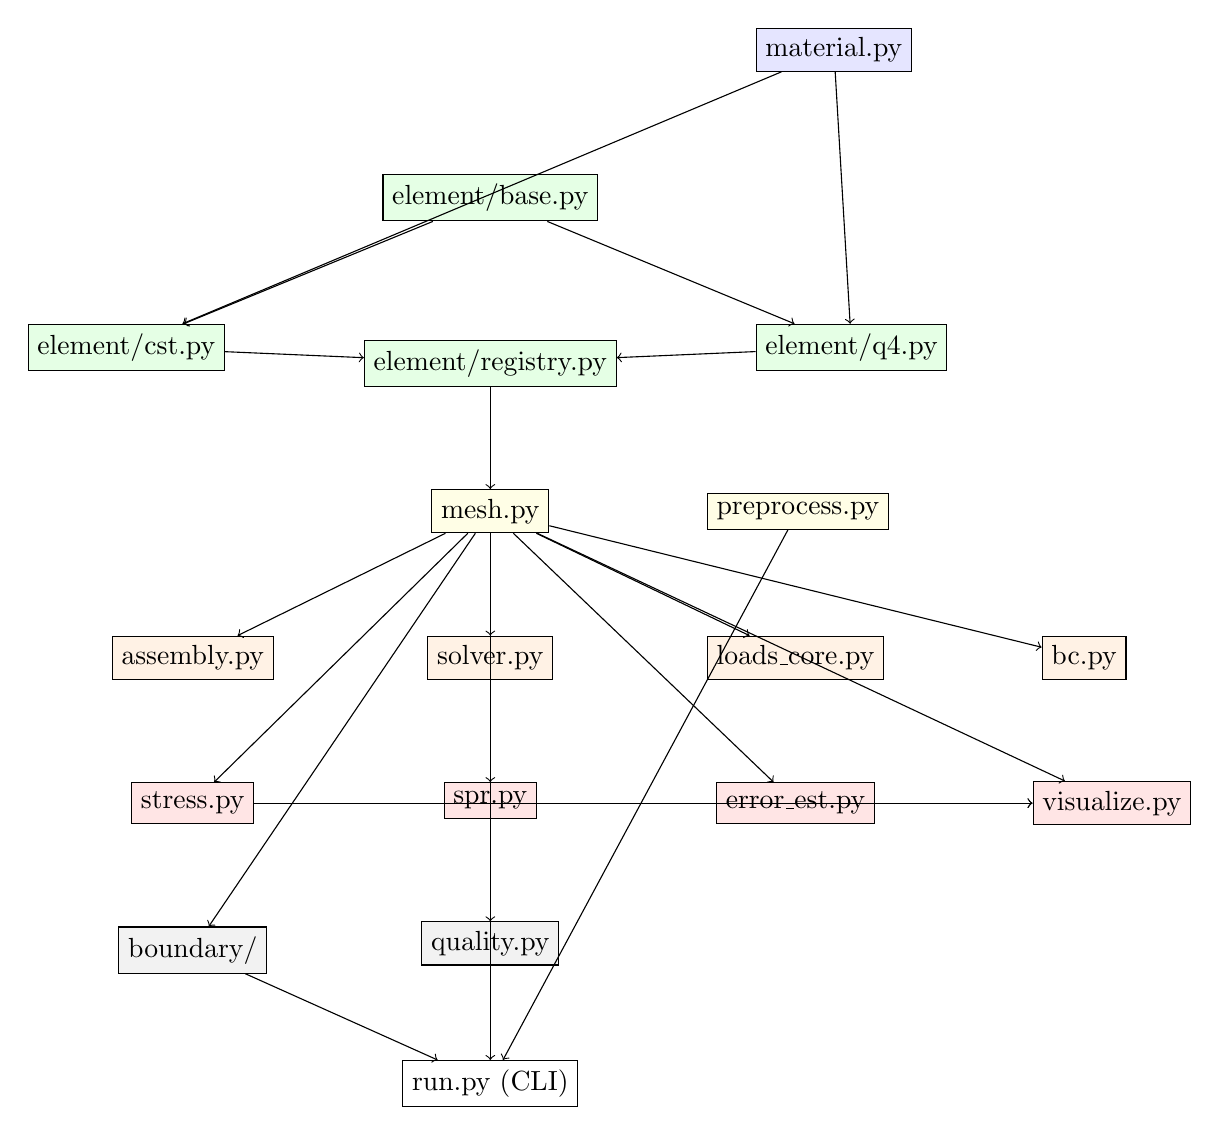
\begin{tikzpicture}[node distance=1.3cm and 2cm, auto]
  % Row 1: material + element protocol
  \node[draw, fill=blue!10] (material) {material.py};
  \node[draw, fill=green!10, below left=of material] (ebase) {element/base.py};
  % Row 2: kernels
  \node[draw, fill=green!10, below left=of ebase] (ecst) {element/cst.py};
  \node[draw, fill=green!10, below right=of ebase] (eq4) {element/q4.py};
  % Row 3: registry
  \node[draw, fill=green!10, below=1.5cm of ebase] (ereg) {element/registry.py};
  % Row 4: data
  \node[draw, fill=yellow!10, below=of ereg] (mesh) {mesh.py};
  \node[draw, fill=yellow!10, right=of mesh] (prep) {preprocess.py};
  % Row 5: solver
  \node[draw, fill=orange!10, below left=of mesh] (assembly) {assembly.py};
  \node[draw, fill=orange!10, below=of mesh] (solver) {solver.py};
  \node[draw, fill=orange!10, below right=of mesh] (loads) {loads\_core.py};
  \node[draw, fill=orange!10, right=of loads] (boundary) {bc.py};
  % Row 6: post
  \node[draw, fill=red!10, below=of assembly] (stress) {stress.py};
  \node[draw, fill=red!10, below=of solver] (spr) {spr.py};
  \node[draw, fill=red!10, below=of loads] (error) {error\_est.py};
  \node[draw, fill=red!10, right=of error] (vis) {visualize.py};
  % Row 7: aux
  \node[draw, fill=gray!10, below=of stress] (bdet) {boundary/};
  \node[draw, fill=gray!10, below=of spr] (quality) {quality.py};
  % Row 8: CLI
  \node[draw, below=1.2cm of quality] (run) {run.py (CLI)};

  % Connections
  \draw[->] (material) -- (ecst);    \draw[->] (material) -- (eq4);
  \draw[->] (ebase) -- (ecst);       \draw[->] (ebase) -- (eq4);
  \draw[->] (ecst) -- (ereg);        \draw[->] (eq4) -- (ereg);
  \draw[->] (ereg) -- (mesh);
  \draw[->] (mesh) -- (assembly);    \draw[->] (mesh) -- (solver);
  \draw[->] (mesh) -- (loads);       \draw[->] (mesh) -- (boundary);
  \draw[->] (mesh) -- (stress);      \draw[->] (mesh) -- (spr);
  \draw[->] (mesh) -- (error);       \draw[->] (mesh) -- (vis);
  \draw[->] (mesh) -- (bdet);        \draw[->] (mesh) -- (quality);
  \draw[->] (prep) -- (run);         \draw[->] (solver) -- (run);
  \draw[->] (stress) -- (vis);       \draw[->] (error) -- (vis);
  \draw[->] (bdet) -- (run);
\end{tikzpicture}
\end{center}

\begin{itemize}
  \item \textbf{蓝色：}材料（所有单元共用）
  \item \textbf{绿色：}单元层（协议 + 实现 + 注册）
  \item \textbf{黄色：}数据层（网格 + 导入）
  \item \textbf{橙色：}求解层（组装 + 求解 + 载荷 + 约束）
  \item \textbf{红色：}后处理（应力 + SPR + Z2 + 可视化）
  \item \textbf{灰色：}辅助（边界检测 + 质量评分）
\end{itemize}

%══════════════════════════════════════════════════════════════
\section{代码设计模式}
%══════════════════════════════════════════════════════════════

\subsection{惰性求值（Lazy Evaluation）}

\texttt{Mesh.build\_connectivity()} 采用惰性求值模式：拓扑数据（node\_to\_elems, elem\_neighbors, boundary\_edges, areas, centroids, element\_dofs）在首次访问时才计算，后续调用直接返回。修改 nodes/elements 后需显式调用 \texttt{invalidate\_cache()}。

好处：Mesh 构造时只做基本校验（不跑拓扑），求解器在需要时才触发计算。避免了“创建 Mesh 就要等很久”的问题。

\subsection{策略模式（Strategy Pattern）}

\texttt{ElementKernel} 是策略模式的典型应用：求解管线（assembly, solver, loads, stress）是\textbf{上下文}，具体的单元类型（CST, Q4）是\textbf{策略}。上下文通过 \texttt{mesh.element\_kernel} 调用策略，不关心具体实现。

\begin{lstlisting}
# 上下文代码（assembly.py）—— 不知道也不关心是什么单元
Ke = mesh.element_kernel.stiffness_batch(mesh)  # 策略方法
dofs = mesh.element_dofs                         # 策略决定的形状
\end{lstlisting}

\subsection{注册表模式（Registry Pattern）}

\texttt{element/registry.py} 维护全局注册表。单元类型通过 \texttt{register\_element(kernel)} 注册自己（含所有别名）。\texttt{get\_element\_kernel(elem\_type)} 按名称查找。重复注册同一键但不同 kernel 实例会报错——防止 import 顺序静默改变单元行为。

\subsection{单一职责分离}

每个模块只做一件事：

\begin{center}
\begin{tabular}{ll}
\hline
\textbf{模块} & \textbf{职责（只有一件）} \\
\hline
mesh.py & 数据容器 + 拓扑构建 \\
material.py & 本构关系（D 矩阵 + von Mises） \\
element/base.py & 定义 kernel 协议 \\
element/cst.py / element/q4.py & 实现具体单元的数学公式 \\
assembly.py & 稀疏矩阵散射 \\
bc.py & 线性代数约束施加 \\
loads\_core.py & 体力/面力/压力积分为等效节点力 \\
solver.py & 流程编排（组装 $\rightarrow$ 求解 $\rightarrow$ 校验） \\
stress.py & 应力恢复（磨平） \\
spr.py & 局部最小二乘拟合 \\
error\_est.py & 误差估计（Z2 + 跳跃 + 残差） \\
visualize.py & 所有 matplotlib 调用 \\
boundary/ & 拓扑、几何谓词、分段与命名 \\
preprocess.py & 文件 I/O 和格式解析 \\
\hline
\end{tabular}
\end{center}

\texttt{run.py} 不包含任何 FEM 算法，也只是进程级入口（编码安全网）——CLI 参数解析在 \texttt{fem2d/cli.py}，输入源解析在 \texttt{fem2d/input\_source.py}，主流程编排与交互输入在 \texttt{fem2d/runner.py}，中文报告在 \texttt{fem2d/reporting.py}。

\subsection{防御性编程}

\textbf{输入校验：}Mesh.\_\_post\_init\_\_ 校验 NaN/Inf、负索引、越界、重复单元、非流形边、材料参数合法性。校验在组装前快速失败，避免难以调试的奇异矩阵错误。

\textbf{原子 I/O：}gmsh\_runner 写入临时文件 $\rightarrow$ 验证拓扑 $\rightarrow$ \texttt{os.replace()} 原子替换。失败时保留旧文件。

\textbf{异常而非静默：}奇异矩阵抛异常（不返回 NaN）、不支持的单元类型抛异常（不跳过）、残差过大抛异常（不让用户拿着错误结果继续分析）。

\subsection{向量化优先}

FEM 的核心操作（刚度组装、应力计算、B 矩阵构造）全部向量化：
\begin{itemize}
  \item 批量 B 矩阵：(ne, 3, n\_dof\_per\_elem) 一次性构造
  \item 批量单刚：\texttt{B.transpose(0,2,1) @ (D @ B)} 无 Python 循环
  \item COO 散射：\texttt{np.broadcast\_to} + 一次 \texttt{coo\_matrix} 调用
\end{itemize}

LIL 参考实现保留用于教学对比（逐标量写入，慢 $\sim 2.5\times$），但生产路径统一使用批量 COO。

%══════════════════════════════════════════════════════════════
\section{加新单元类型的步骤}
%══════════════════════════════════════════════════════════════

以加 Q8（八节点四边形）为例：

\begin{enumerate}[leftmargin=*]
  \item 新建 \texttt{element\_q8.py}，实现 \texttt{ElementKernel} 的 8 个抽象方法
  \item 在文件末尾调用 \texttt{register\_element(Q8Element())}
  \item 在 \texttt{element\_registry.py} 加一行 \texttt{from .element\_q8 import Q8, Q8Element}
  \item 在 \texttt{preprocess.py} 的 \texttt{\_VALID\_ELEMENTS} 中加 \texttt{"CPS8": 8}
  \item \texttt{assembly.py} / \texttt{solver.py} / \texttt{loads\_core.py} / \texttt{stress.py} / \texttt{error\_est.py} / \texttt{boundary\_detect.py}：\textbf{无需修改}
\end{enumerate}

\end{document}
